\documentclass[conference]{IEEEtran}
\usepackage[T1]{fontenc}
\usepackage{cite}
\usepackage{amsmath,amssymb}
\usepackage{graphicx}
\usepackage{booktabs}
\usepackage[hidelinks]{hyperref}
\hypersetup{pdftitle={Campaign-Level Adversarial Stress Testing in a Synthetic UPI-Inspired Fraud Laboratory},pdfauthor={Perplexity Computer}}
\begin{document}
\title{Campaign-Level Adversarial Stress Testing in a Synthetic UPI-Inspired Fraud Laboratory}
\author{\IEEEauthorblockN{Author details pending researcher approval}
\IEEEauthorblockA{Academic review draft; institution and contact to be supplied}}
\maketitle
\begin{abstract}
Transaction-level fraud scores do not directly describe whether an evolving sequence reaches a transfer target before intervention. We present an auditable, synthetic research laboratory for campaign-level stress testing, with a local dashboard, recorded ledger transitions, constrained attacker policies and independently reconstructed results. A retained exploratory pilot compares static, rule-adaptive, learned, label-blind learned and zero-Q policies against newly fitted XGBoost and Random Forest detectors in nine independent blocks. A declared gradual-escalation mechanism is excluded from registered detector-development data, but this narrow exclusion does not establish unseen real-world fraud detection. Across 7,200 evaluated attack campaigns, 3,539 reach their target. Legitimate gradual-escalation mimics are blocked in 48.278 percent of XGBoost episodes and 12.806 percent of Random Forest episodes, despite no observed blocks on ordinary benign test episodes. Rule-feedback differences favor the adaptive rule on this held-out mechanism; learning-control differences are detector-dependent. The contribution is reproducible research infrastructure and an adverse synthetic case study, not a new detector algorithm, universal reinforcement-learning advantage, or evidence of real-world UPI effectiveness.
\end{abstract}
\begin{IEEEkeywords}
fraud detection, adversarial evaluation, synthetic data, reinforcement learning, reproducibility
\end{IEEEkeywords}

\section{Introduction and Problem Statement}
Fraud evaluation depends on more than classification accuracy. Operational supervision timing, class imbalance and drift affect what detector results mean \cite{dalpozzolo}. In a sequence of attempted transfers, an early intervention may prevent later actions, while an alert that permits a transfer has a different consequence from a block. A campaign endpoint is therefore a useful complementary measurement: does a simulated actor reach a defined target under a specified detector and resource contract?

This laboratory is UPI-inspired rather than connected to Unified Payments Interface infrastructure. It uses synthetic accounts, virtual payment-address strings, ledger updates and model scores; it does not implement a banking network, victim behavior, investigation process or settlement recovery. Its name must not be read as deployment validation. Existing legacy experiments and a later matched pilot answer different questions and are kept separate.

We ask: (RQ1) what campaign outcomes occur under matched policy constraints; (RQ2) does excluding a specified synthetic mechanism from detector development imply useful discrimination when benign episodes exhibit the same mechanism; and (RQ3) can the outputs, policy state and numerical claims be independently checked? These questions are exploratory. The retained study was not a powered, independently custodied confirmatory lockbox experiment.

\section{Related Work}
Financial detector evasion is established research. Carminati et al. evaluate attacks against banking fraud systems under different knowledge conditions using real bank datasets \cite{carminati}. Fraud-RLA applies reinforcement learning to credit-card detector evasion \cite{fraudrla}. Its accessible earlier preprint formulates a single-step partially observed problem, uses PPO with continuous correlated actions and compares statistical mimicry attacks \cite{fraudrlav1}. Its preprint methods are not assumed identical to the unread journal full text. Our tabular policy and multi-transaction ledger campaign differ, but neither learning attackers nor financial evasion originates here.

Sequence-aware fraud detection also predates this work: an HMM can model normal cardholder operation sequences \cite{hmm}. PaySim demonstrates synthetic mobile-money simulation grounded in available transaction statistics; its 2016 paper leaves malicious injection and detector evaluation outside that paper's scope \cite{paysim}. Synthetic finance requires separate consideration of realism, similarity and privacy \cite{assefa}; reproducibility alone does not certify any of these.

Concept-drift research distinguishes changing distributions and predictive relationships over time \cite{gama}. Our imposed benign mechanism shift is not a longitudinal drift-adaptation experiment. TESSERACT illustrates the importance of realistic space/time splits in another security domain \cite{tesseract}, while Henderson et al. emphasize variance and reproducibility in RL comparisons \cite{henderson}. These works motivate disciplined measurement, not a claim that their findings validate this simulator.

\section{Research Gap and Contributions}
The bounded gap addressed by this engineering study is an inspectable connection between policy decisions, ledger effects, intervention outcomes and artifact-bound experimental provenance. The package combines: (i) explicit campaign stopping and monetary bookkeeping; (ii) matched online constraints for five policies; (iii) registered exclusion of one synthetic grammar and ancestry; (iv) benign mechanism-shift controls; and (v) reconstruction and local visualization of the evidence. We claim an implemented combination and a documented failure case, not priority over all literature or superiority to published methods.

The literature matrix accompanies the source package and identifies abstract-only evidence and missing methodological detail. No published attack was reimplemented on common data. Accordingly, literature comparison is qualitative, not a performance ranking.

\section{System Architecture and Implementation}
The existing Python engine separates campaign generation, attackers, detector adapters, a synthetic environment and campaign execution. XGBoost \cite{xgboost} and Random Forest \cite{rf} are reused baselines. The ledger records proposed amounts, actual simulated source debit, decisions, feature values and termination. Checkpoint files preserve tabular policies and fitted model identities.

A lightweight local workstation consists of a standard-library Python HTTP backend and a vanilla JavaScript interface. Eleven sections cover overview, execution, logs, results, detector and attacker comparisons, campaign detail, artifacts, validation, exports and settings. It invokes fixed command templates with validated arguments, one active job, approved output roots and process-group cancellation. It has no arbitrary shell, user-selected executable, publication or Gate C endpoint. It binds loopback by default and is not an internet-facing security-certified service.

The integration adds portable hash-verified evidence restoration and strengthens the pilot verifier to reject one directory reused as main/repeat/reload, wrong run roles and mismatched configurations. These are software/evidence integrity improvements, not new detector-training experiments. Original raw records and model bytes remain unchanged.

\section{Threat Model and Problem Formulation}
The simulated attacker controls legal amount/pacing choices, observes permitted feedback and seeks a target transfer before the first BLOCK. It does not alter the fitted detector or access true test labels. Online resource limits are common across pilot arms. Offline learned-policy training costs are reported separately and are not equal to static-policy construction costs.

For campaign \(i\), let \(T_i\) be its target, \(m_{it}\) actual simulated debit on proposal \(t\), and \(B_i\) its stopping index. Completion is
\begin{equation}
C_i=\mathbf{1}\left\{\sum_{t\leq B_i}m_{it}\geq T_i\right\}.
\end{equation}
BLOCK produces zero debit for that proposal and terminates the campaign; FLAG can still debit funds. The detector is fixed during evaluation. This is a restricted partial-observation simulation, not a strategic equilibrium, convergence proof or universal attacker model.

\section{Data and Synthetic Mechanism Generation}
The legacy implementation supports high-value burst, slow drain, gradual escalation and beneficiary hopping. Its corrected retained study has 1,152 campaigns and 4,161 transactions across three seeds. Excluding workloads from attacker training does not establish exclusion from the historical detectors' training; that ancestry remains unverified.

The separate pilot evaluates high-value burst (HVB) and gradual escalation (GE). HVB begins at INR 15,000, with later nominal proposals of INR 8,000 or 15,000. GE begins at INR 1,000 and progresses by at most one band through INR 1,000, 3,000, 8,000 and 15,000, with bounded repeated proposals. Final proposals are clipped to remaining target/budget; grammar checks retain nominal-band identity.

Each of nine independent blocks registers 1,000 balanced-by-episode fit episodes, 400 allowed-family validation episodes, 1,000 ordinary-benign calibration episodes and two distinct 400-episode benign test strata. Row balance need not equal episode balance. Role-specific seed namespaces separate generation, fitting, policy training and evaluation. GE generation, derived ancestry and nontrivial matching prefixes are excluded from fit, validation and calibration; signature-positive ordinary-benign candidates are quarantined without relabeling.

The four causal features are amount, hour of day, trailing one-hour source velocity and new-beneficiary indicator. No fitted scaler or SMOTE is used in this pilot. Exact feature-value overlap across roles is not equivalent to mechanism ancestry overlap. This holdout is a registered synthetic exclusion, not proof that arbitrary real fraud is unseen.

One benign test stratum follows ordinary behavior; the other is labeled legitimate but exhibits the GE mechanism. It probes an intentionally challenging ambiguity in this representation. The generator is not statistically calibrated to real UPI transaction logs, and these labels do not establish how actual legitimate users behave.

\section{Detectors, Thresholds and Attacker Policies}
Each block fits an XGBoost model with 100 trees and depth 4 and a Random Forest with 150 trees and depth 8, using fixed hyperparameters and single-threaded fitting. Detector-development records, actual feature/label inputs, model hashes and episode memberships are retained.

Thresholds are chosen from independent ordinary-benign episode-maximum scores using deterministic order statistics and tie handling. Nominal empirical calibration budgets are at most 0.5\% any-BLOCK and 2.5\% any-alert. They are not population guarantees, and no GE test label selects thresholds or hyperparameters. An impossible supported threshold is an error rather than a silent all-ALLOW sentinel.

All five arms share family-specific legal masks, 300/1,200-second pacing, fixed source/sink, INR 20,000--40,000 targets, target-sized gross budget, initial balance, 30 proposals and an 86,400-second duration limit. Static and rule policies use the same kernel with neutral versus actual last-label feedback. Learned RL receives progress/horizon bins and the previous decision; label-blind RL masks the explicit label state but still receives detector-dependent training rewards. It is therefore not fully feedback-free. Zero-Q starts without learned values and uses the common legal action/tie-breaking rules.

Both learned arms train 300 HVB episodes per detector/block with common training contexts and exploration streams. Tabular updates use \(\alpha=0.25\), \(\gamma=0.95\), legally masked bootstraps, no terminal bootstrap, and decaying training exploration. Reward is
\begin{align}
r_t={}&3\min(m_t/T,1)+2C_t-\mathbf{1}_{\mathrm{BLOCK}}\nonumber\\
&-0.2\mathbf{1}_{\mathrm{FLAG}}-0.02
-0.5\mathbf{1}_{\mathrm{failed\ horizon,\ not\ BLOCK}} .
\end{align}
The policy uses zero exploration during evaluation, while tied best actions retain seeded tie-breaking. Evaluation reads missing Q rows without inserting them and checks persisted policy equality after episodes. Frozen model bytes are also checked. There is no claim of optimal learning or complete observability.

\section{Experimental Protocol and Statistical Analysis}
Each block evaluates 40 paired contexts per mechanism, shared across detectors and five arms, yielding \(9\times40\times2\times2\times5=7,200\) attack campaigns. Learned training comprises 10,800 episodes and 18 detector fits. Repeat runs with identical seeds test reproducibility, not independent replication. Checkpoint-only reload performs evaluation without fitting or policy training.

The independent replication unit is the block, not a transaction, campaign row or repeat directory. Completion is summarized by arm/detector/mechanism, with block standard deviations. Three GE contrasts per detector are descriptive: rule minus static, RL minus label-blind RL, and RL minus zero-Q. The current reconstruction uses paired block percentile bootstrap intervals with 10,000 draws and seed 20261026. These are exploratory, unadjusted intervals across six contrasts, not multiplicity-controlled discoveries.

Nine blocks were retained as a pilot allocation, not a prospective power calculation. Five absolute percentage points is only an effect-of-interest sensitivity reference. A confirmatory sample would require researcher-approved operating points, paired discordance and between-block variance estimates, an explicit multiplicity policy and a genuinely untouched lockbox. No such follow-up is claimed here.

\section{Metrics and Evidence Traceability}
Completion is completed/attempted campaigns. Transaction counts include evaluated decisions, separately ALLOW, FLAG and BLOCK. Gross simulated debit is the sum of recorded transferred amounts, calculated in integer paise; it is neither actual victim loss nor money saved. Blocked proposed amounts are not observed savings.

First BLOCK measures elapsed simulated seconds to intervention; first FLAG-or-BLOCK measures time to first alert. Conditional means must be accompanied by event counts because no-event campaigns are censored by their stopping/horizon mechanism. This paper does not turn those means into unbiased time-to-event estimates. Benign false-block rate is episodes with maximum score at or above BLOCK threshold divided by episodes in that benign stratum.

Detector AUC is not campaign completion. Historical AUC claims are not independently adopted, and allowed-family validation AUC is not held-out-GE test performance. Every project result here is generated from retained raw records by \texttt{scripts/reproduce\_paper.py}. Its reconstruction manifest lists source hashes; the bundled evidence archive stores exact recorded bytes.

\section{Results}
\subsection{Attack Campaign Outcomes}
The retained full pilot contains 3,539 completed campaigns out of 7,200, or 49.153\% when pooled solely as a descriptive workload total. It has 28,895 evaluated transactions: 24,634 ALLOW, 600 FLAG and 3,661 BLOCK. Gross simulated source debit is INR 192,300,996.32. The pooled completion rate does not estimate a real fraud prevalence or strategy-independent population effect.

\begin{table}[t]
\caption{Pilot campaign completion (\%). Each cell: 360 campaigns in nine blocks. HVB is allowed in development; GE is the declared held-out mechanism.}
\label{tab:completion}\centering
\setlength{\tabcolsep}{3pt}
\begin{tabular}{llrrrrr}\toprule
Detector&Family&Static&Rule&RL&Blind RL&Zero Q\\\midrule
XGB & HVB & 3.611 & 3.333 & 3.333 & 4.444 & 4.167 \\
XGB & GE & 1.667 & 75.278 & 43.333 & 42.222 & 50.833 \\
RF & HVB & 58.333 & 56.667 & 74.444 & 75.278 & 48.056 \\
RF & GE & 71.111 & 100.000 & 91.944 & 89.722 & 85.278 \\
\bottomrule\end{tabular}

\end{table}

Table~\ref{tab:completion} and Fig.~\ref{fig:completion} show strong task dependence. On GE, rule minus static is 73.611 percentage points for XGBoost and 28.889 for Random Forest. Exploratory paired block intervals are [65.556,82.222] and [24.444,33.611], respectively. Those contrasts concern this rule kernel and online constraints, not arbitrary adaptive attackers.

RL minus label-blind RL on GE is 1.111 points for XGBoost and 2.222 for Random Forest; intervals are [-5.000,6.667] and [-4.444,8.889]. RL minus zero-Q is -7.500 points for XGBoost and 6.667 for Random Forest, with intervals [-16.944,3.056] and [2.778,10.000]. These unadjusted pilot summaries neither establish universal learning superiority nor prove equality where intervals include zero.

\begin{figure*}[t]\centering
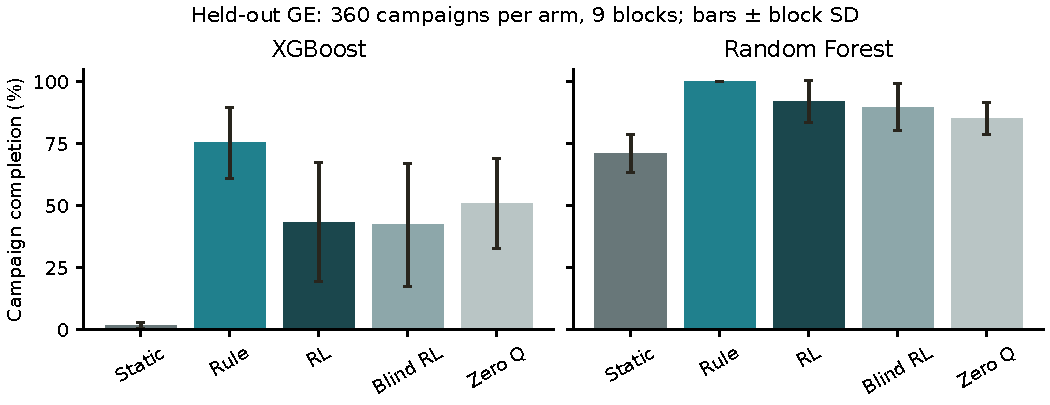
\includegraphics[width=\textwidth]{figures/completion.pdf}
\caption{GE completion in the retained pilot. Error bars show one between-block standard deviation, not confidence intervals; nine independent blocks per arm/detector. The upper margin accommodates variability beyond the 100\% mean ceiling.}
\label{fig:completion}
\end{figure*}

\subsection{Benign Mechanism Shift}
Both detectors have zero observed BLOCK among 3,600 ordinary-benign test episodes each. This is not a certified zero population false-block rate. On legitimate GE mimics, XGBoost blocks 1,738/3,600 (48.278\%) and Random Forest blocks 461/3,600 (12.806\%). Any-alert rates on this stratum are 1,862/3,600 (51.722\%) and 536/3,600 (14.889\%). These outcomes are adverse evidence against interpreting mechanism exclusion as reliable fraud discrimination.

\begin{figure}[t]\centering
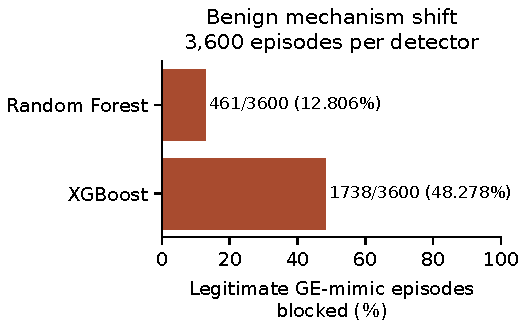
\includegraphics[width=\columnwidth]{figures/benign_shift.pdf}
\caption{Observed legitimate GE-mimic false blocking in the retained pilot; 3,600 episodes per detector in nine blocks. Ordinary-benign BLOCK is zero observed, not a population guarantee.}
\label{fig:benign}
\end{figure}

\subsection{Legacy Study and Reconstruction}
The corrected legacy study is not pooled into Table~\ref{tab:completion}. Its known-workload static and rule-adaptive completion is 100\% for both detectors; its records do not establish the historical ``adaptation paradox.'' Its comparisons retain different action/pacing/clipping and training-cost conditions.

The current strengthened pilot verifier passes 1,012,673 checks and replays 30,985 recorded TD updates from retained artifacts. A separate analysis passes 44,608 hash/arithmetic/record checks, reproducing the pilot totals and the legacy campaign/transaction counts. These are evidence integrity checks, not new statistical replications or proof that the simulator represents deployed UPI.

\section{Discussion of Findings and Failures}
The benign mimic result is the most important warning. The registered exclusion is real within the synthetic protocol, yet a mechanism associated with attack evaluation also appears in legitimate test episodes. The four-feature detector may not distinguish intent under that construction. This is a plausible interpretation of the representation and experimental design, not an identified causal diagnosis; attributing the rate to a particular feature would require controlled ablations or external evidence.

The rule contrast demonstrates that feedback can change observed campaign completion for the implemented kernel. It does not imply adaptive behavior must always help: HVB results and mixed RL controls contradict an unqualified statement. Floors and ceilings also restrict what these tasks reveal.

Integration exposed a verifier weakness accepting a reused directory and a dashboard portability error rejecting approved nested local-state artifacts. Both were corrected with regression tests. An initial HTTP demonstration attempt failed before repeat execution; it is preserved alongside the successful continuation. No failed attempt was converted into a passing record, and no engine reward or historical model was retuned for favorable outcomes.

\section{Threats to Validity}
Internal validity is limited by unequal offline policy costs, constrained action grammars, partially observed state and reward-mediated information in the label-blind arm. Common online masks do not make every aspect of training equivalent. Artifact provenance supports registered membership and fitted inputs but not unavailable historical detector ancestry.

Statistical validity is limited by nine blocks, related contexts, six unadjusted contrasts, synthetic labels and no prospective power analysis. Repeat/reload equality demonstrates deterministic reproduction within the tested environment, not additional independent evidence. Threshold calibration is finite and ordinary-benign conditional.

External validity is limited by four features, only two mechanisms in the matched pilot, no real UPI logs, no human investigation, no production latency or distributed service behavior, and no external detector deployment. Synthetic distribution shift is not a longitudinal real-world drift estimate. Software tests validate exercised behavior, not scientific generalization.

\section{Ethical and Responsible-Use Considerations}
The package is intended for offline defensive research with synthetic identifiers, not attempts against payment services. Models use pickle-compatible artifacts; load only trusted hash-verified project files. The workstation must stay local; no real customer identifiers, credentials or payment traffic should enter it without separate approval and safeguards.

This is an AI-assisted draft prepared for researcher review. Human authors must verify arguments, approve attribution and comply with university and venue policies. AI-content and similarity checks are pending approved external verification; no measured percentage or threshold compliance is claimed. Author identities, institution, venue/page limit and final submission approval are outstanding.

\section{Conclusion and Future Work}
An inspectable campaign pipeline can connect attacker choices to intervention and synthetic ledger effects while exposing failures hidden by aggregate success rates. The retained pilot supports a narrow mechanism-exclusion claim and a substantial benign mechanism-shift failure, not general unseen-fraud validation. A qualified engineering contribution is the integrated, reproducible evidence package and local workstation.

Future work requires approved real data, better-supported feature/behavior assumptions, training-cost-matched comparisons, representation ablations and a powered, independently custodied evaluation. Those experiments are not part of this integration. Scientific validity is assessed only to the extent supported by the recorded audit and analyses; Gate C remains HOLD.

\bibliographystyle{IEEEtran}
\bibliography{references}
\end{document}
